\section{Introduction}


In the last few decades, quantum computing has become a very active field of research. A significant reason for its success is its promise to outperform classical computers in specific tasks. The most famous example of such a computational speedup is Shor's algorithm \cite{shor1994algorithms}, as it allows factorizing large numbers in polynomial time.  The algorithm allows for a significant speedup compared to the best-known classical algorithm (GNFS), which takes sub-exponential time.
Another example is Grover's algorithm \cite{grover1996fast}, which allows for searching entries in an unsorted database in $\mathcal{O}(\sqrt{N})$ time. Grover's algorithm provides a quadratic speedup compared to the classical $\mathcal{O}(N)$ search time. \cite{nielsen2010quantum}

Usually, those algorithms are described in a high-level language, the so-called (quantum-)circuit model. This model allows to intuitively reason about quantum algorithms because every operation applied to the quantum state is represented by a single gate. However, this model does not consider the restrictions of real quantum computers \cite{equivalence_checking_tum} and needs to be compiled into a circuit that can be executed on a real quantum computer. This process is called \textit{quantum circuit compilation}.

\subsection{Quantum Circuit Compilation}

Real quantum computers come with a set of restrictions. For example, the allowed gates are typically limited to a small set of universal gates (like the Clifford+T gate set). Furthermore, the connectivity of the qubits is limited. These restrictions imply that not every operation can be applied to every pair of qubits. Consequently, the original circuit needs to be \textit{compiled} into an equivalent circuit that can be executed on the specific quantum computer while still respecting the restrictions. \cite{equivalence_checking_tum}

\begin{figure}
    \centering
    \begin{quantikz}
        \lstick{$\ket{c_1}$} & \ctrl{1}  & \qw\\
        \lstick{$\ket{c_2}$} & \ctrl{1} & \qw \\
        \lstick{$\ket{t}$}   & \targ{}  & \qw
    \end{quantikz}
    \caption{The Toffoli gate.}
    \label{fig:toffoli_gate}
\end{figure}

\begin{figure}
    \centering
    \begin{quantikz}[row sep=0.3cm, column sep=0.2cm]
        \lstick{$\ket{c_1}$} & \qw& \qw &\qw & \ctrl{2}& \qw & \qw & \qw & \ctrl{2} & \ctrl{1} & \gate{T} & \ctrl{1} & \qw \\
        \lstick{$\ket{c_2}$} & \qw&  \ctrl{1}  & \qw  & \qw & \qw & \ctrl{1} & \gate{T} & \qw  & \targ{} & \gate{T^\dagger} & \targ{} & \qw \\
        \lstick{$\ket{t}$} &\gate{H}& \targ{}  & \gate{T^\dagger} & \targ{} & \gate{T} & \targ{} & \gate{T^\dagger} & \targ{} & \gate{T} & \gate{H} & \qw & \qw\\
    \end{quantikz}
    \caption{Decomposition of the Toffoli gate in the Clifford+T gate set.}
    \label{fig:toffoli_decomposition}
\end{figure}


Many quantum computers only support the Clifford+T gate set because it is an approximately universal gate set, meaning that every circuit can be simulated to a certain degree of accuracy \cite{nielsen2010quantum}. Furthermore, this set allows for an efficient, fault-tolerant implementation using surface code error correction \cite{kissinger2020TCount}.

\subsection{Compilation of the Toffoli Gate}

In this section, we will look at the compilation of the Toffoli gate using the Clifford+T gate set. We first look at the original Toffoli gate, shown in figure \ref{fig:toffoli_gate}. As the Toffoli gate doesn't exist in the Clifford+T gate set, it needs to be adapted in order to be executed on a real quantum computer. The compilation of the Toffoli gate into the Clifford+T gate set is shown in figure \ref{fig:toffoli_decomposition}.

\subsection{Quantum Circuit Optimization}

Notice how the amount of gates increased significantly. This increase in complexity is a common problem in quantum circuit compilation, as it means that the compiled circuit will be slower. This is a massive problem since the execution time of the new circuit can exceed the coherence time of the qubits, thus making the computation useless \cite{nielsen2010quantum}.

Circuit Optimizers can help to mitigate this problem, as they try to reduce the number of gates in a circuit. Optimizers often work by applying rewrite rules to the circuit, which keep the circuit equivalent to the original, but reduce the number of gates. An important metric for simplifying quantum circuits is the so-called \textit{T-Count}. The T-Count is the number of T gates in a circuit. Since the T-Gate is a non-Clifford gate, it is costly to simulate and requires orders of magnitudes more resources than the traditional Clifford gates \cite{kissinger2020TCount}. Therefore, reducing the T-Count is a crucial step in quantum circuit optimization.

\subsection{Drawbacks of Classical Circuit Optimization}

There are many different approaches to quantum circuit optimization. The most basic approach is to apply a set of rewrite rules directly to the logic-gate representation of the circuit. This approach is called \textit{gate-level optimization}. \cite{namyross2018automated}

This trivial approach is typically very inefficient, as there exist many possible rewrite rules (Some of them are shown in figure \ref{fig:rewrite_rules_classical}). Furthermore, rewrite rules are typically not independent of each other, as applying a rewrite rule can introduce new opportunities for different rewrite rules, thus making it very hard to find an optimal solution \cite{alexkissinger2020introductionzx}.

\begin{figure}[h]
    \centering
    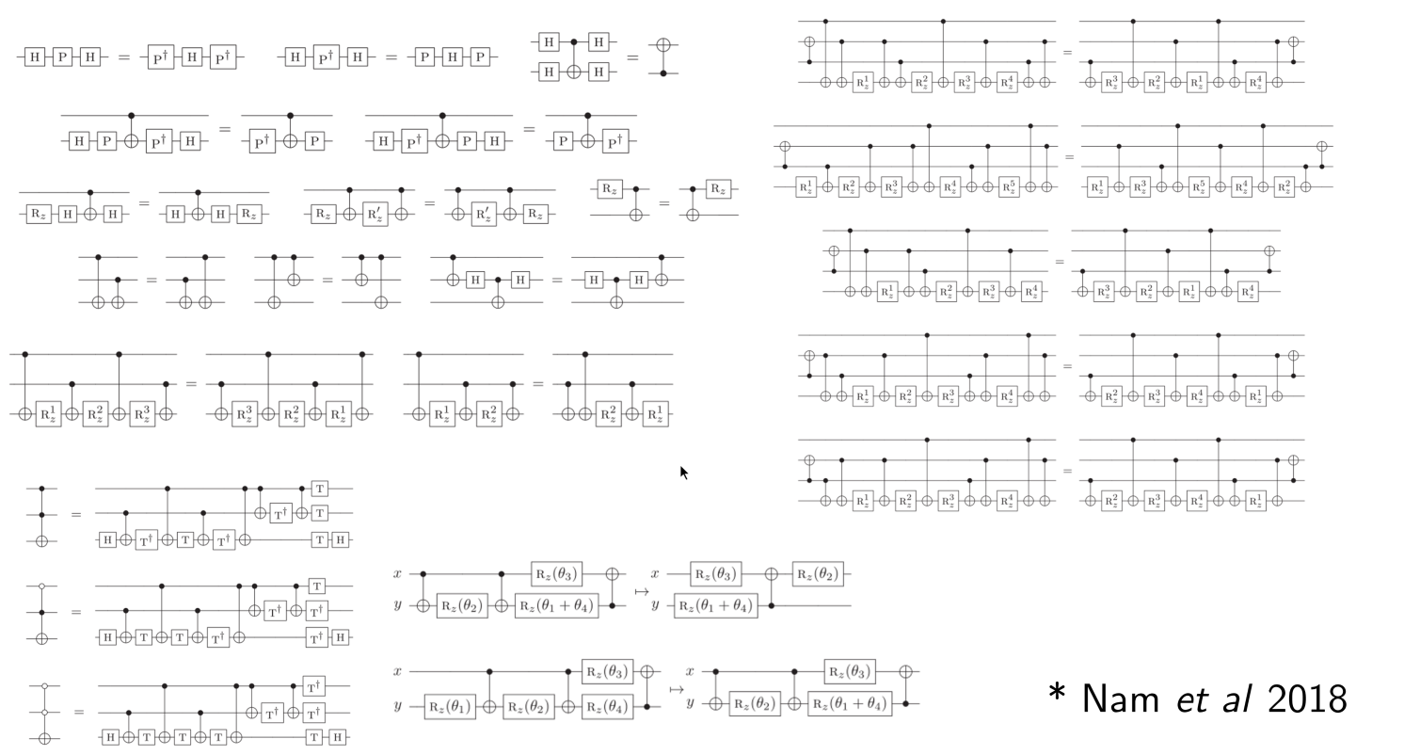
\includegraphics[width=\linewidth]{images/rewrite_rules_classical.png}
    \caption{Small subset of rewrite rules for classical circuit optimization
            {\cite{alexkissinger2020introductionzx}}}
    \label{fig:rewrite_rules_classical}
\end{figure}


\subsection{Quantum Circuit Optimization using the ZX-Calculus}

A more efficient approach for quantum circuit optimization is found in the ZX-Calculus. The ZX-Calculus is a graphical language for quantum computing, differing from the logic-gate representation by using connected nodes to represent operations on qubits. This new representation utilizes way fewer \textit{gate-types} than the classical representation; consequently, there are fewer rewrite rules to consider in each step.

ZX-Calculus has been kickstarted by Coecke and Duncan in 2008 \cite{Coecke2007graphicalcalculus}. Since then, it has been used to prove many exciting results in quantum computing. It was initially used in the field of Measurement-Based Quantum Computing (MBQC) \cite{duncan2012graphical}. But recently, it has found wide application in quantum circuit optimization and verification \cite{vandewetering2020zxcalculus}.